% SPDX-License-Identifier: CC-BY-4.0
\documentclass[11pt,letterpaper]{article}

\usepackage[T1]{fontenc}
\usepackage{amsmath,amssymb}
\usepackage{tikz}
\usepackage{pgfplots}
\pgfplotsset{compat=1.18}
\usepackage{algorithm}
\usepackage{algpseudocode}
\usepackage{booktabs}
\usepackage{enumitem}
\usepackage[hidelinks]{hyperref}

\newcommand{\N}{\mathbb{N}}
\newcommand{\Z}{\mathbb{Z}}
\newcommand{\Q}{\mathbb{Q}}
\newcommand{\R}{\mathbb{R}}
\newcommand{\C}{\mathbb{C}}
\newcommand{\Map}[3]{#1 \colon #2 \to #3}
\newcommand{\Mod}[1]{#1\text{-}\mathrm{Mod}}
\newcommand{\GroupHom}{\mathrm{Hom}_{\mathbf{Grp}}}
\newcommand{\RingHom}{\mathrm{Hom}_{\mathbf{Ring}}}

\newtheorem{theorem}{Theorem}
\newtheorem{lemma}[theorem]{Lemma}
\newtheorem{corollary}[theorem]{Corollary}
\newtheorem{definition}[theorem]{Definition}
\newtheorem{remark}[theorem]{Remark}
\newenvironment{proof}{\noindent\textit{Proof.}}{\hfill\(\square\)}

\title{Generalized Collatz Library}
\author{}
\date{\today}

\begin{document}
\maketitle

\begin{abstract}
This article records the first, second, and third homomorphism theorems in three algebraic settings: groups, unital rings, and unital left modules. Each theorem is stated in full, proved from the universal property of the quotient, and accompanied by a commutative diagram drawn in TikZ. The statements follow Lang \cite{Lang02}, Hungerford \cite{Hungerford74}, Atiyah--Macdonald \cite{AtiyahMacdonald69}, and Dummit--Foote \cite{DummitFoote04}. The text is the typesetting standard for the Generalized Collatz Library: Computer Modern Roman under pdfLaTeX, letter paper, eleven point, PascalCase macros, AMS alpha citations, and no hardcoded spacing commands. Matching Lean proofs live in \texttt{Templates/lean/}. The homomorphism theorems apply to the additive linear part \(x\mapsto qx\) of a residue-class affine map. The translation \(c\) must be tracked separately: \(x\mapsto qx+c\) is not an additive homomorphism unless \(c=0\) in the codomain.
\end{abstract}

\section{Conventions}

Composition is written \((\varphi\circ\psi)(x)=\varphi(\psi(x))\). The identity element of a group \(G\) is \(e_G\), abbreviated \(e\) when \(G\) is clear. A group homomorphism \(\Map{\varphi}{G}{H}\) satisfies \(\varphi(xy)=\varphi(x)\varphi(y)\) for all \(x,y\in G\); it follows that \(\varphi(e_G)=e_H\) and \(\varphi(x^{-1})=\varphi(x)^{-1}\).

Rings are associative and unital. A ring homomorphism \(\Map{\varphi}{R}{S}\) satisfies \(\varphi(a+b)=\varphi(a)+\varphi(b)\), \(\varphi(ab)=\varphi(a)\varphi(b)\), and \(\varphi(1_R)=1_S\). Kernels of ring homomorphisms are two-sided ideals. Modules are unital left modules over a unital ring \(R\): \(1_R\cdot m=m\) for every \(m\in M\). An \(R\)-module homomorphism is an additive map commuting with scalar multiplication.

The image of \(\varphi\) is written \(\operatorname{im}\varphi\). The kernel is \(\ker\varphi\). Normal subgroups are written \(N\trianglelefteq G\). The coset of \(g\in G\) modulo \(N\) is \(gN\). The quotient group (respectively ring, module) is \(G/N\) (respectively \(R/I\), \(M/N\)).

The first homomorphism theorem is the comparison between a morphism and the quotient by its kernel. The second identifies a sum-intersection quotient with a restricted quotient. The third identifies an iterated quotient with a single quotient. In each algebraic category the three statements are instances of the same diagram chase, with the relevant notion of kernel replacing the others.

\begin{definition}
Let \(\Map{\varphi}{G}{H}\) be a group homomorphism. The \emph{kernel} of \(\varphi\) is \(\ker\varphi=\{g\in G:\varphi(g)=e_H\}\). The \emph{image} of \(\varphi\) is \(\operatorname{im}\varphi=\{\varphi(g):g\in G\}\).
\end{definition}

\begin{lemma}
\label{lem:kernel-normal}
If \(\Map{\varphi}{G}{H}\) is a group homomorphism, then \(\ker\varphi\trianglelefteq G\) and \(\operatorname{im}\varphi\leq H\).
\end{lemma}

\begin{proof}
Let \(K=\ker\varphi\). If \(a,b\in K\), then \(\varphi(ab)=\varphi(a)\varphi(b)=e_H e_H=e_H\), so \(ab\in K\). Also \(\varphi(a^{-1})=\varphi(a)^{-1}=e_H^{-1}=e_H\), so \(a^{-1}\in K\). Thus \(K\leq G\). For \(g\in G\) and \(k\in K\),
\[
\varphi(gkg^{-1})=\varphi(g)\varphi(k)\varphi(g)^{-1}=\varphi(g)e_H\varphi(g)^{-1}=e_H,
\]
so \(gkg^{-1}\in K\). Hence \(K\trianglelefteq G\). If \(\varphi(g),\varphi(h)\in\operatorname{im}\varphi\), then \(\varphi(g)\varphi(h)=\varphi(gh)\) and \(\varphi(g)^{-1}=\varphi(g^{-1})\), so \(\operatorname{im}\varphi\leq H\).
\end{proof}

The same computation, with additive notation and with scalars, yields that kernels of ring homomorphisms are two-sided ideals and that kernels of module homomorphisms are submodules. Those variants are recorded in the sections that use them.

\section{Groups}

Let \(G\) and \(H\) be groups. Write \(\GroupHom(G,H)\) for the set of group homomorphisms from \(G\) to \(H\). The quotient homomorphism \(\Map{\pi}{G}{G/N}\) associated to \(N\trianglelefteq G\) is \(\pi(g)=gN\). It is surjective, and \(\ker\pi=N\).

\subsection{First homomorphism theorem}

\begin{theorem}[First homomorphism theorem for groups]
\label{thm:group-first}
Let \(\Map{\varphi}{G}{H}\) be a group homomorphism. Let \(K=\ker\varphi\). There exists a unique group isomorphism \(\Map{\overline{\varphi}}{G/K}{\operatorname{im}\varphi}\) such that \(\varphi=\iota\circ\overline{\varphi}\circ\pi\), where \(\Map{\pi}{G}{G/K}\) is the quotient map and \(\Map{\iota}{\operatorname{im}\varphi}{H}\) is the inclusion. Explicitly, \(\overline{\varphi}(gK)=\varphi(g)\). In particular \(G/\ker\varphi\cong\operatorname{im}\varphi\).
\end{theorem}

\begin{proof}
Define \(\overline{\varphi}(gK)=\varphi(g)\). If \(gK=g'K\), then \(g^{-1}g'\in K\), so
\[
\varphi(g)^{-1}\varphi(g')=\varphi(g^{-1}g')=e_H.
\]
Hence \(\varphi(g)=\varphi(g')\), and \(\overline{\varphi}\) is well-defined. For the homomorphism property,
\[
\overline{\varphi}((gK)(g'K))=\overline{\varphi}(gg'K)=\varphi(gg')=\varphi(g)\varphi(g')=\overline{\varphi}(gK)\overline{\varphi}(g'K).
\]
If \(\overline{\varphi}(gK)=e_H\), then \(\varphi(g)=e_H\), so \(g\in K\) and \(gK=K\). Thus \(\overline{\varphi}\) is injective. If \(h\in\operatorname{im}\varphi\), then \(h=\varphi(g)=\overline{\varphi}(gK)\) for some \(g\in G\), so \(\overline{\varphi}\) is surjective. Therefore \(\overline{\varphi}\) is an isomorphism.

Uniqueness follows from surjectivity of \(\pi\): any morphism \(\psi\) with \(\varphi=\iota\circ\psi\circ\pi\) satisfies \(\psi(gK)=\varphi(g)=\overline{\varphi}(gK)\). The identity \(\varphi=\iota\circ\overline{\varphi}\circ\pi\) is immediate from the formula.
\end{proof}

\begin{center}
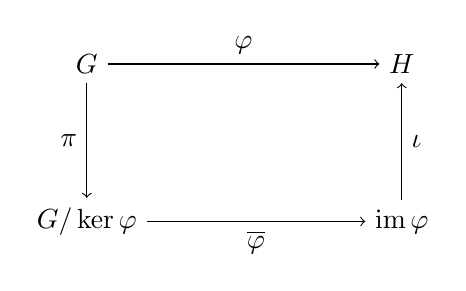
\begin{tikzpicture}
\node (G) at (0,2) {$G$};
\node (H) at (4,2) {$H$};
\node (Q) at (0,0) {$G/\ker\varphi$};
\node (I) at (4,0) {$\operatorname{im}\varphi$};
\draw[->] (G) -- node[above] {$\varphi$} (H);
\draw[->] (G) -- node[left] {$\pi$} (Q);
\draw[->] (Q) -- node[below] {$\overline{\varphi}$} (I);
\draw[->] (I) -- node[right] {$\iota$} (H);
\end{tikzpicture}
\end{center}

\begin{remark}
The first homomorphism theorem is the statement that every group homomorphism factors uniquely as a surjection, an isomorphism, and an injection. For the reduction \(\Z/12\Z\to\Z/4\Z\), the kernel is \(\{0,4,8\}\), the image has four elements, and each fibre has three elements. Taking \(\varphi\) injective yields \(G\cong\operatorname{im}\varphi\), so injective homomorphisms are isomorphic onto their images.
\end{remark}

\subsection{Second homomorphism theorem}

Let \(H\leq G\) and \(N\trianglelefteq G\). The product \(HN=\{hn:h\in H,\, n\in N\}\) is a subgroup of \(G\): if \(h_1 n_1, h_2 n_2\in HN\), then
\[
(h_1 n_1)(h_2 n_2)=h_1 h_2 (h_2^{-1} n_1 h_2) n_2\in HN,
\]
using that \(N\) is normal, and \((hn)^{-1}=n^{-1}h^{-1}=h^{-1}(h n^{-1} h^{-1})\in HN\). Moreover \(N\trianglelefteq HN\) because \(N\trianglelefteq G\) and \(N\subseteq HN\). The intersection \(H\cap N\) is a subgroup of \(H\). It is normal in \(H\): if \(h\in H\) and \(x\in H\cap N\), then \(h x h^{-1}\in H\) because \(H\) is a subgroup, and \(h x h^{-1}\in N\) because \(N\) is normal in \(G\).

\begin{theorem}[Second homomorphism theorem for groups]
\label{thm:group-second}
Let \(H\leq G\) and \(N\trianglelefteq G\). Then \(HN\leq G\), \(N\trianglelefteq HN\), \(H\cap N\trianglelefteq H\), and
\[
HN/N \cong H/(H\cap N).
\]
\end{theorem}

\begin{proof}
Define \(\Map{\varphi}{H}{HN/N}\) by \(\varphi(h)=hN\). This is a homomorphism because
\[
\varphi(h_1 h_2)=(h_1 h_2)N=(h_1 N)(h_2 N)=\varphi(h_1)\varphi(h_2).
\]
It is surjective: an arbitrary coset of \(N\) in \(HN\) has the form \((hn)N=hN=\varphi(h)\). The kernel is
\[
\ker\varphi=\{h\in H:hN=N\}=\{h\in H:h\in N\}=H\cap N.
\]
Theorem~\ref{thm:group-first} yields \(H/(H\cap N)\cong\operatorname{im}\varphi=HN/N\).
\end{proof}

\begin{center}
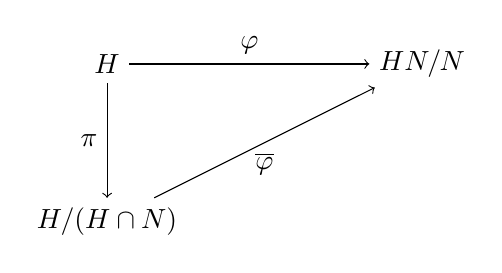
\begin{tikzpicture}
\node (H) at (0,2) {$H$};
\node (Q) at (4,2) {$HN/N$};
\node (K) at (0,0) {$H/(H\cap N)$};
\draw[->] (H) -- node[above] {$\varphi$} (Q);
\draw[->] (H) -- node[left] {$\pi$} (K);
\draw[->] (K) -- node[below] {$\overline{\varphi}$} (Q);
\end{tikzpicture}
\end{center}

\begin{remark}
If \(G\) is abelian, every subgroup is normal, so the second homomorphism theorem applies to every pair of subgroups \(H,N\leq G\), with \(HN=H+N\) in additive notation, and \((H+N)/N\cong H/(H\cap N)\). This is the form used for residue-class groups \(\Z/d\Z\) and for the abelian groups that carry Collatz-type maps \(n\mapsto qn+c\).
\end{remark}

\subsection{Third homomorphism theorem}

\begin{theorem}[Third homomorphism theorem for groups]
\label{thm:group-third}
Let \(N\trianglelefteq G\) and let \(H\) be a subgroup of \(G\) with \(N\leq H\trianglelefteq G\). Then \(H/N\trianglelefteq G/N\) and
\[
(G/N)/(H/N) \cong G/H.
\]
\end{theorem}

\begin{proof}
Define \(\Map{\varphi}{G/N}{G/H}\) by \(\varphi(gN)=gH\). If \(gN=g'N\), then \(g^{-1}g'\in N\subseteq H\), so \(gH=g'H\). Thus \(\varphi\) is well-defined. It is a homomorphism:
\[
\varphi((gN)(g'N))=\varphi(gg'N)=(gg')H=(gH)(g'H)=\varphi(gN)\varphi(g'N).
\]
It is surjective because every coset \(gH\) is \(\varphi(gN)\). The kernel is
\[
\ker\varphi=\{gN:gH=H\}=\{gN:g\in H\}=H/N.
\]
In particular \(H/N=\ker\varphi\trianglelefteq G/N\). Theorem~\ref{thm:group-first} yields \((G/N)/(H/N)\cong G/H\).
\end{proof}

\begin{center}
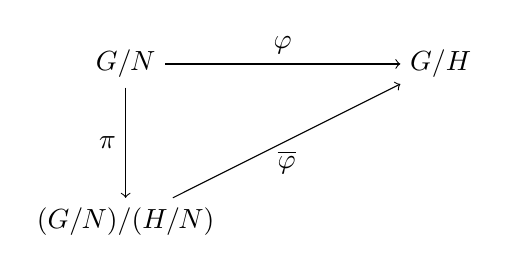
\begin{tikzpicture}
\node (GN) at (0,2) {$G/N$};
\node (GH) at (4,2) {$G/H$};
\node (Q) at (0,0) {$(G/N)/(H/N)$};
\draw[->] (GN) -- node[above] {$\varphi$} (GH);
\draw[->] (GN) -- node[left] {$\pi$} (Q);
\draw[->] (Q) -- node[below] {$\overline{\varphi}$} (GH);
\end{tikzpicture}
\end{center}

\begin{remark}
The third homomorphism theorem says that collapsing \(N\) and then collapsing the image of \(H\) is the same as collapsing \(H\) in one step. In the correspondence theorem, subgroups of \(G/N\) are in bijection with subgroups of \(G\) containing \(N\); the third homomorphism theorem identifies the quotient by the subgroup corresponding to \(H\) with \(G/H\).
\end{remark}

\section{Rings}

Let \(R\) and \(S\) be unital rings. Write \(\RingHom(R,S)\) for unital ring homomorphisms. An additive subgroup \(I\subseteq R\) is a two-sided ideal if \(rI\subseteq I\) and \(Ir\subseteq I\) for all \(r\in R\). The quotient ring \(R/I\) has multiplication \((a+I)(b+I)=ab+I\), which is well-defined precisely because \(I\) is a two-sided ideal. The quotient map \(\Map{\pi}{R}{R/I}\), \(\pi(r)=r+I\), is a unital ring homomorphism with kernel \(I\).

\begin{lemma}
\label{lem:ring-kernel}
If \(\Map{\varphi}{R}{S}\) is a unital ring homomorphism, then \(\ker\varphi\) is a two-sided ideal of \(R\) and \(\operatorname{im}\varphi\) is a unital subring of \(S\).
\end{lemma}

\begin{proof}
Additively, \(\ker\varphi\) is a subgroup of \(R\) by Lemma~\ref{lem:kernel-normal} applied to the underlying abelian groups. If \(x\in\ker\varphi\) and \(r\in R\), then \(\varphi(rx)=\varphi(r)\varphi(x)=\varphi(r)\cdot 0_S=0_S\) and \(\varphi(xr)=\varphi(x)\varphi(r)=0_S\), so \(rx,xr\in\ker\varphi\). Thus \(\ker\varphi\) is a two-sided ideal. The image contains \(0_S=\varphi(0_R)\) and \(1_S=\varphi(1_R)\). If \(y=\varphi(a)\) and \(z=\varphi(b)\) lie in the image, then \(y+z=\varphi(a+b)\), \(-y=\varphi(-a)\), and \(yz=\varphi(ab)\) also lie in the image. Hence the image is a unital subring.
\end{proof}

\subsection{First homomorphism theorem}

\begin{theorem}[First homomorphism theorem for rings]
\label{thm:ring-first}
Let \(\Map{\varphi}{R}{S}\) be a unital ring homomorphism. Let \(I=\ker\varphi\). There exists a unique unital ring isomorphism \(\Map{\overline{\varphi}}{R/I}{\operatorname{im}\varphi}\) such that \(\varphi=\iota\circ\overline{\varphi}\circ\pi\), where \(\pi\) is the quotient map and \(\iota\) is the inclusion of the image. Explicitly, \(\overline{\varphi}(r+I)=\varphi(r)\). In particular \(R/\ker\varphi\cong\operatorname{im}\varphi\).
\end{theorem}

\begin{proof}
Define \(\overline{\varphi}(r+I)=\varphi(r)\). If \(r+I=r'+I\), then \(r-r'\in I\), so \(\varphi(r)-\varphi(r')=\varphi(r-r')=0_S\) and \(\varphi(r)=\varphi(r')\). Thus \(\overline{\varphi}\) is well-defined. Additivity and multiplicativity are inherited from \(\varphi\):
\begin{align*}
\overline{\varphi}((r+I)+(r'+I))&=\overline{\varphi}(r+r'+I)=\varphi(r+r')=\varphi(r)+\varphi(r'),\\
\overline{\varphi}((r+I)(r'+I))&=\overline{\varphi}(rr'+I)=\varphi(rr')=\varphi(r)\varphi(r').
\end{align*}
Also \(\overline{\varphi}(1_R+I)=\varphi(1_R)=1_S\). If \(\overline{\varphi}(r+I)=0_S\), then \(r\in I\), so \(\overline{\varphi}\) is injective. Surjectivity onto \(\operatorname{im}\varphi\) is the definition of the image. Uniqueness is the same as in Theorem~\ref{thm:group-first}: \(\pi\) is surjective.
\end{proof}

\begin{center}
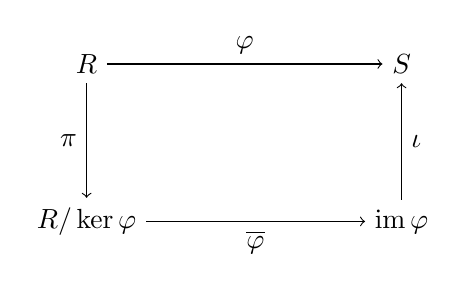
\begin{tikzpicture}
\node (R) at (0,2) {$R$};
\node (S) at (4,2) {$S$};
\node (Q) at (0,0) {$R/\ker\varphi$};
\node (I) at (4,0) {$\operatorname{im}\varphi$};
\draw[->] (R) -- node[above] {$\varphi$} (S);
\draw[->] (R) -- node[left] {$\pi$} (Q);
\draw[->] (Q) -- node[below] {$\overline{\varphi}$} (I);
\draw[->] (I) -- node[right] {$\iota$} (S);
\end{tikzpicture}
\end{center}

\begin{remark}
The Chinese remainder theorem is the first homomorphism theorem applied to \(\Map{\varphi}{R}{R/I\times R/J}\), \(\varphi(r)=(r+I,r+J)\), when \(I+J=R\). Then \(\ker\varphi=I\cap J\) and \(\varphi\) is surjective, so \(R/(I\cap J)\cong R/I\times R/J\). For \(R=\Z\), \(I=m\Z\), \(J=n\Z\) with \(\gcd(m,n)=1\), this is \(\Z/mn\Z\cong\Z/m\Z\times\Z/n\Z\).
\end{remark}

\subsection{Second homomorphism theorem}

Let \(S\subseteq R\) be a unital subring and let \(I\) be a two-sided ideal of \(R\). The sum \(S+I=\{s+i:s\in S,\, i\in I\}\) is a unital subring of \(R\): it contains \(1_R=1_S+0\), and
\[
(s_1+i_1)(s_2+i_2)=s_1 s_2 + s_1 i_2 + i_1 s_2 + i_1 i_2\in S+I
\]
because \(s_1 s_2\in S\) and the remaining three terms lie in \(I\). The set \(I\) is a two-sided ideal of \(S+I\). The intersection \(S\cap I\) is a two-sided ideal of \(S\): if \(s\in S\) and \(x\in S\cap I\), then \(sx,xs\in S\) and \(sx,xs\in I\).

\begin{theorem}[Second homomorphism theorem for rings]
\label{thm:ring-second}
Let \(S\) be a unital subring of a unital ring \(R\) and let \(I\) be a two-sided ideal of \(R\). Then \(S+I\) is a unital subring of \(R\), \(I\) is a two-sided ideal of \(S+I\), \(S\cap I\) is a two-sided ideal of \(S\), and
\[
(S+I)/I \cong S/(S\cap I).
\]
\end{theorem}

\begin{proof}
Define \(\Map{\varphi}{S}{(S+I)/I}\) by \(\varphi(s)=s+I\). This is a unital ring homomorphism: it preserves addition and multiplication because those operations in the quotient are induced from \(R\), and \(\varphi(1_S)=1_S+I=1_{S+I}+I\). It is surjective because \((s+i)+I=s+I=\varphi(s)\). The kernel is
\[
\ker\varphi=\{s\in S:s+I=I\}=\{s\in S:s\in I\}=S\cap I.
\]
Theorem~\ref{thm:ring-first} yields \(S/(S\cap I)\cong(S+I)/I\).
\end{proof}

\begin{center}
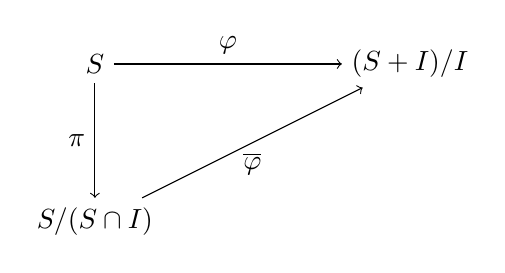
\begin{tikzpicture}
\node (S) at (0,2) {$S$};
\node (Q) at (4,2) {$(S+I)/I$};
\node (K) at (0,0) {$S/(S\cap I)$};
\draw[->] (S) -- node[above] {$\varphi$} (Q);
\draw[->] (S) -- node[left] {$\pi$} (K);
\draw[->] (K) -- node[below] {$\overline{\varphi}$} (Q);
\end{tikzpicture}
\end{center}

\begin{remark}
Take \(R=\Z\times\Z\), \(S=\{(n,n):n\in\Z\}\), and \(I=2\Z\times3\Z\). For any \((x,y)\in R\), put \(n=4y-3x\). Then \((x,y)-(n,n)\in I\), so \(S+I=R\). The intersection is \(S\cap I=\{(6k,6k):k\in\Z\}\). Thus the theorem gives
\[
\Z/2\Z\times\Z/3\Z\cong\Z/6\Z.
\]
A unital subring of \(\Z\) must contain \(1\) and therefore equals \(\Z\); \(n\Z\) is not a unital subring of \(\Z\) for \(n>1\).
\end{remark}

\subsection{Third homomorphism theorem}

\begin{theorem}[Third homomorphism theorem for rings]
\label{thm:ring-third}
Let \(I\subseteq J\) be two-sided ideals of a unital ring \(R\). Then \(J/I\) is a two-sided ideal of \(R/I\) and
\[
(R/I)/(J/I) \cong R/J.
\]
\end{theorem}

\begin{proof}
Define \(\Map{\varphi}{R/I}{R/J}\) by \(\varphi(r+I)=r+J\). If \(r+I=r'+I\), then \(r-r'\in I\subseteq J\), so \(r+J=r'+J\). Thus \(\varphi\) is well-defined. It is a unital ring homomorphism because addition and multiplication of cosets are induced from \(R\), and \(\varphi(1_R+I)=1_R+J\). It is surjective: \(r+J=\varphi(r+I)\). The kernel is
\[
\ker\varphi=\{r+I:r+J=J\}=\{r+I:r\in J\}=J/I.
\]
Hence \(J/I\) is a two-sided ideal of \(R/I\). Theorem~\ref{thm:ring-first} yields \((R/I)/(J/I)\cong R/J\).
\end{proof}

\begin{center}
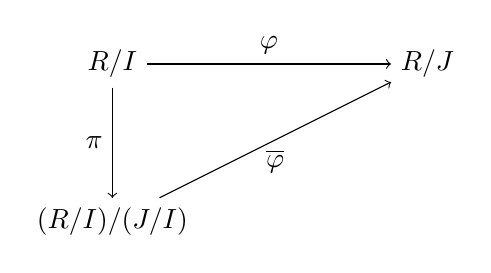
\begin{tikzpicture}
\node (RI) at (0,2) {$R/I$};
\node (RJ) at (4,2) {$R/J$};
\node (Q) at (0,0) {$(R/I)/(J/I)$};
\draw[->] (RI) -- node[above] {$\varphi$} (RJ);
\draw[->] (RI) -- node[left] {$\pi$} (Q);
\draw[->] (Q) -- node[below] {$\overline{\varphi}$} (RJ);
\end{tikzpicture}
\end{center}

\begin{remark}
Iterated residue rings collapse. If \(n\) divides \(m\) in \(\Z\), then
\[
(\Z/m\Z)/(n\Z/m\Z)\cong\Z/n\Z,
\]
which is the third homomorphism theorem with \(R=\Z\), \(I=m\Z\), \(J=n\Z\). This is the algebraic content of reducing a congruence modulo \(m\) further modulo \(n\).
\end{remark}

\section{Modules}

Let \(R\) be a unital ring and let \(M,N\) be unital left \(R\)-modules. An \(R\)-module homomorphism \(\Map{\varphi}{M}{N}\) is a map of abelian groups with \(\varphi(r\cdot m)=r\cdot\varphi(m)\) for all \(r\in R\) and \(m\in M\). Submodules are additive subgroups closed under the \(R\)-action. The quotient \(M/K\) by a submodule \(K\) is an \(R\)-module via \(r\cdot(m+K)=rm+K\). The category of left \(R\)-modules is written \(\Mod{R}\).

\begin{lemma}
\label{lem:mod-kernel}
If \(\Map{\varphi}{M}{N}\) is an \(R\)-module homomorphism, then \(\ker\varphi\) is a submodule of \(M\) and \(\operatorname{im}\varphi\) is a submodule of \(N\).
\end{lemma}

\begin{proof}
Additively, \(\ker\varphi\) is a subgroup. If \(x\in\ker\varphi\) and \(r\in R\), then \(\varphi(rx)=r\varphi(x)=r\cdot 0=0\), so \(rx\in\ker\varphi\). If \(\varphi(m),\varphi(m')\in\operatorname{im}\varphi\), then \(\varphi(m)+\varphi(m')=\varphi(m+m')\) and \(r\varphi(m)=\varphi(rm)\), so the image is a submodule.
\end{proof}

\subsection{First homomorphism theorem}

\begin{theorem}[First module theorem]
\label{thm:mod-first}
Let \(\Map{\varphi}{M}{N}\) be a homomorphism of left \(R\)-modules, and put \(K=\ker\varphi\). There is a unique \(R\)-module isomorphism
\[
\Map{\overline{\varphi}}{M/K}{\operatorname{im}\varphi}
\quad\text{with}\quad
\varphi=\iota\circ\overline{\varphi}\circ\pi,
\]
where \(\pi\) is the quotient map and \(\iota\) is the inclusion. Explicitly, \(\overline{\varphi}(m+K)=\varphi(m)\). Thus \(M/\ker\varphi\cong\operatorname{im}\varphi\).
\end{theorem}

\begin{proof}
Define \(\overline{\varphi}(m+K)=\varphi(m)\). If \(m+K=m'+K\), then \(m-m'\in K\), so \(\varphi(m)=\varphi(m')\). Additivity is inherited from \(\varphi\). For scalars,
\[
\overline{\varphi}(r\cdot(m+K))=\overline{\varphi}(rm+K)=\varphi(rm)=r\varphi(m)=r\cdot\overline{\varphi}(m+K).
\]
Injectivity: \(\overline{\varphi}(m+K)=0\) implies \(m\in K\). If \(n\in\operatorname{im}\varphi\), choose \(m\) with \(\varphi(m)=n\). Then \(\overline{\varphi}(m+K)=n\), proving surjectivity. Uniqueness follows from surjectivity of \(\pi\).
\end{proof}

\begin{center}
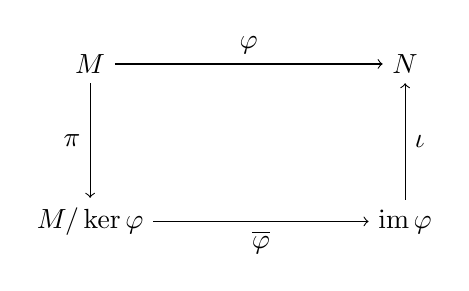
\begin{tikzpicture}
\node (M) at (0,2) {$M$};
\node (N) at (4,2) {$N$};
\node (Q) at (0,0) {$M/\ker\varphi$};
\node (I) at (4,0) {$\operatorname{im}\varphi$};
\draw[->] (M) -- node[above] {$\varphi$} (N);
\draw[->] (M) -- node[left] {$\pi$} (Q);
\draw[->] (Q) -- node[below] {$\overline{\varphi}$} (I);
\draw[->] (I) -- node[right] {$\iota$} (N);
\end{tikzpicture}
\end{center}

\begin{remark}
For \(R=\Z\), left \(\Z\)-modules are abelian groups, so Theorem~\ref{thm:mod-first} specialises to Theorem~\ref{thm:group-first} in additive notation. For \(R=\Z/d\Z\), modules are abelian groups with exponent dividing \(d\), so the additive linear parts of residue-class affine maps can be treated as module homomorphisms.
\end{remark}

\subsection{Second homomorphism theorem}

Let \(A,B\subseteq M\) be submodules. The sum \(A+B=\{a+b:a\in A,\, b\in B\}\) is a submodule. The intersection \(A\cap B\) is a submodule of \(A\) and of \(B\).

\begin{theorem}[Second module theorem]
\label{thm:mod-second}
Let \(A,B\leq M\) be submodules of a left \(R\)-module. Their sum and intersection are submodules, and
\[
(A+B)/B \cong A/(A\cap B).
\]
\end{theorem}

\begin{proof}
Define \(\Map{\varphi}{A}{(A+B)/B}\) by \(\varphi(a)=a+B\). This is an \(R\)-module homomorphism:
\[
\varphi(a+a')=(a+a')+B=(a+B)+(a'+B),\qquad
\varphi(ra)=ra+B=r\cdot(a+B).
\]
It is surjective because \((a+b)+B=a+B=\varphi(a)\). The kernel is
\[
\ker\varphi=\{a\in A:a+B=B\}=\{a\in A:a\in B\}=A\cap B.
\]
Theorem~\ref{thm:mod-first} yields \(A/(A\cap B)\cong(A+B)/B\).
\end{proof}

\begin{center}
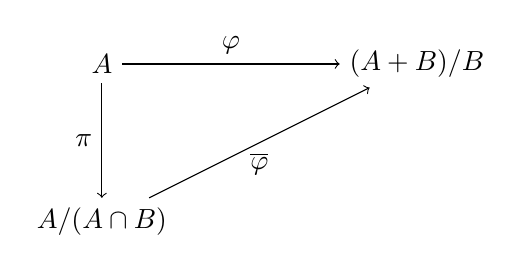
\begin{tikzpicture}
\node (A) at (0,2) {$A$};
\node (Q) at (4,2) {$(A+B)/B$};
\node (K) at (0,0) {$A/(A\cap B)$};
\draw[->] (A) -- node[above] {$\varphi$} (Q);
\draw[->] (A) -- node[left] {$\pi$} (K);
\draw[->] (K) -- node[below] {$\overline{\varphi}$} (Q);
\end{tikzpicture}
\end{center}

\begin{remark}
For a left ideal \(\mathfrak{a}\) of \(R\), submodules of the cyclic left module \(R/\mathfrak{a}\) correspond to left ideals containing \(\mathfrak{a}\). This is a module statement; a left ideal need not define a quotient ring. For \(M=\Z\), \(A=4\Z\), and \(B=6\Z\), the sum is \(2\Z\), the intersection is \(12\Z\), and both \(2\Z/6\Z\) and \(4\Z/12\Z\) are cyclic groups of order \(3\).
\end{remark}

\subsection{Third homomorphism theorem}

\begin{theorem}[Third module theorem]
\label{thm:mod-third}
Let \(N\subseteq P\) be submodules of a left \(R\)-module \(M\). The image \(P/N\) in \(M/N\) is a submodule, and
\[
(M/N)/(P/N) \cong M/P.
\]
\end{theorem}

\begin{proof}
Define \(\Map{\varphi}{M/N}{M/P}\) by \(\varphi(m+N)=m+P\). If \(m+N=m'+N\), then \(m-m'\in N\subseteq P\), so \(m+P=m'+P\). Thus \(\varphi\) is well-defined. It is an \(R\)-module homomorphism because
\[
\begin{aligned}
\varphi((m+N)+(m'+N))&=(m+m')+P,\\
\varphi(r\cdot(m+N))&=rm+P=r\cdot\varphi(m+N).
\end{aligned}
\]
It is surjective: \(m+P=\varphi(m+N)\). The kernel is
\[
\ker\varphi=\{m+N:m+P=P\}=\{m+N:m\in P\}=P/N.
\]
Hence \(P/N\) is a submodule of \(M/N\). Theorem~\ref{thm:mod-first} yields \((M/N)/(P/N)\cong M/P\).
\end{proof}

\begin{center}
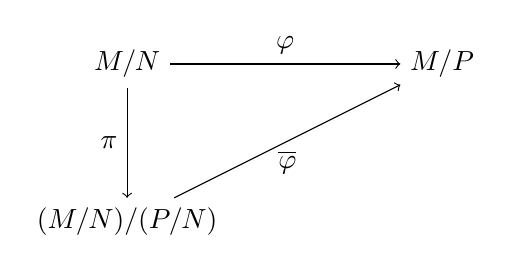
\begin{tikzpicture}
\node (MN) at (0,2) {$M/N$};
\node (MP) at (4,2) {$M/P$};
\node (Q) at (0,0) {$(M/N)/(P/N)$};
\draw[->] (MN) -- node[above] {$\varphi$} (MP);
\draw[->] (MN) -- node[left] {$\pi$} (Q);
\draw[->] (Q) -- node[below] {$\overline{\varphi}$} (MP);
\end{tikzpicture}
\end{center}

\begin{remark}
The third homomorphism theorem for modules is the Noether isomorphism that identifies successive quotients. In homological algebra it is the reason that a filtration \(0\subseteq N\subseteq P\subseteq M\) yields an exact comparison between \(M/P\) and the quotient of \(M/N\) by \(P/N\). For Collatz residue modules, collapsing a progression nested inside another progression is a single quotient, not two.
\end{remark}

\section{Induced maps}

The three theorems produce an induced isomorphism from a homomorphism and compatible subobjects. For a finitely generated domain with known kernel \(K\), the following construction specifies its values on quotient generators. It does not compute the kernel or solve a word problem.

\begin{algorithm}
\caption{InducedIsomorphism}
\begin{algorithmic}[1]
\Require homomorphism \(\varphi\) with known kernel \(K\)
\Require domain generators \(g_1,\ldots,g_n\)
\Ensure induced isomorphism onto \(\operatorname{im}\varphi\)
\For{\(i \gets 1\) \textbf{to} \(n\)}
	\State \(\overline{\varphi}([g_i]_K) \gets \varphi(g_i)\)
\EndFor
\State Extend using the homomorphism law; the first theorem verifies the relations
\State \Return \(\overline{\varphi}\)
\end{algorithmic}
\end{algorithm}

Table~\ref{tab:iso} summarises the three identifications in each category.

\begin{table}[htbp]
\centering
\caption{Homomorphism theorems.}
\label{tab:iso}
\begin{tabular}{lll}
\toprule
Setting & Theorem & Identification \\
\midrule
Groups & First & \(G/\ker\varphi\cong\operatorname{im}\varphi\) \\
       & Second & \(HN/N\cong H/(H\cap N)\) \\
       & Third & \((G/N)/(H/N)\cong G/H\) \\
\midrule
Rings & First & \(R/\ker\varphi\cong\operatorname{im}\varphi\) \\
      & Second & \((S+I)/I\cong S/(S\cap I)\) \\
      & Third & \((R/I)/(J/I)\cong R/J\) \\
\midrule
Modules & First & \(M/\ker\varphi\cong\operatorname{im}\varphi\) \\
        & Second & \((A+B)/B\cong A/(A\cap B)\) \\
        & Third & \((M/N)/(P/N)\cong M/P\) \\
\bottomrule
\end{tabular}
\end{table}

The proofs share a skeleton. Construct a homomorphism out of the object that is to be the left-hand side of the desired isomorphism, with values in the right-hand side. Prove well-definedness from the containment of kernels or of the smaller subobject. Prove that the map is a homomorphism from the algebraic operations. Compute the kernel and identify it with the denominator of the left-hand side. Invoke the first homomorphism theorem, or, in the first theorem itself, verify injectivity and surjectivity directly.

\begin{enumerate}[label=\arabic*.]
\item First theorem: the kernel is exactly the fibre of the identity, so the induced map on the quotient is injective, and it is surjective onto the image by construction.
\item Second theorem: restrict the quotient map of the sum (or product) to the smaller subobject; the kernel is the intersection.
\item Third theorem: the map sends a coset modulo the smaller subobject to a coset modulo the larger subobject; its kernel is the intermediate quotient.
\end{enumerate}

\section{Preamble package check}

The following macros and plot exercise the remaining preamble packages. Keep this template self-contained.

Macros: \(\N,\Z,\Q,\R,\C\), \(\Map{\varphi}{\Z}{\Z}\), \(\Mod{R}\), \(\GroupHom\), \(\RingHom\).

\begin{center}
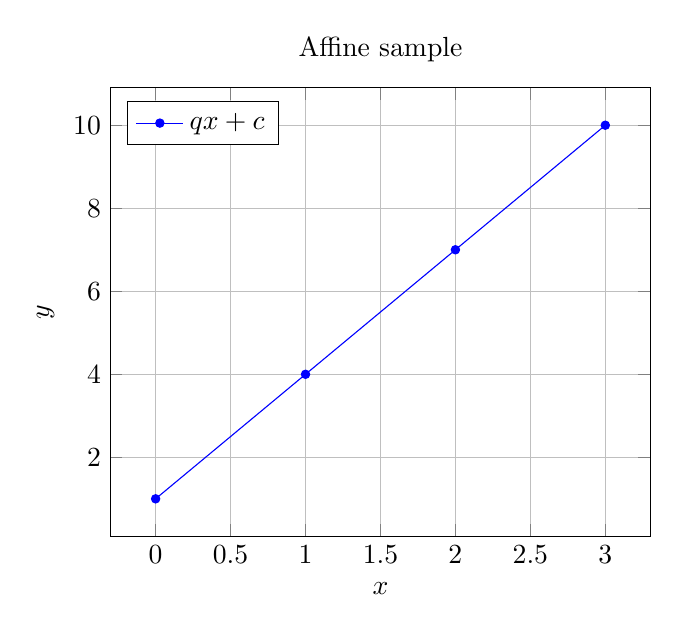
\begin{tikzpicture}
\begin{axis}[
	xlabel={$x$},
	ylabel={$y$},
	title={Affine sample},
	legend pos=north west,
	grid=major
]
\addplot[blue,mark=*,mark size=1.5pt] coordinates {(0,1) (1,4) (2,7) (3,10)};
\addlegendentry{$qx+c$}
\end{axis}
\end{tikzpicture}
\end{center}

\bibliographystyle{amsalpha}
\bibliography{Template}

\end{document}
